\documentclass{report}
\usepackage{amsmath, amssymb, amsthm}
\usepackage{geometry}
\geometry{a4paper, margin=1in}
\usepackage{float}
\usepackage{tikz}
\usetikzlibrary{calc, decorations.pathreplacing}
\usepackage{pgfplots}
\pgfplotsset{compat=1.18}
\usepackage{xcolor}
\usepackage{tcolorbox}
\tcbuselibrary{theorems}
\usepackage{eurosym}
\usepackage{fancyhdr}
\usepackage{booktabs}

\begin{document}

\pagestyle{fancy}
\fancyhf{}
\rhead{Report 1 \;|\; Stochastic Methods for Finance \;|\; \thepage}
\renewcommand{\headrulewidth}{0.4pt}
\setlength{\headheight}{14pt}

\section{Methodology: Step-by-Step Excel Implementation}
The MP Materials (MP) Call option was valued in Excel using a One-Step Binomial Model calibrated on market and historical data.

\textit{Every step implementation can be checked in the provided file:} \texttt{Report1\_Quartucci\_Davide.xlsx}

\paragraph{Step 1: Finding Data \& Daily Returns}
Using Yahoo Finance, the Spot Price ($S_0$), the ATM Strike Price ($K$), and the Bid and Ask quotes of the selected 3-month and 6-month Call options were collected. In Excel, the market benchmark was computed as the Mid-Price:
$$P_{mid} = \frac{P_{bid} + P_{ask}}{2}$$

\paragraph{Step 2: Historical Data Extraction and Excel Integration}
To respect the \textit{Matching Principle}, the volatility input was estimated on historical windows consistent with option maturity. Two datasets of daily closing prices ($P_t$) were downloaded from Yahoo Finance:
\begin{itemize}
    \item A \textbf{3-month} historical sample.
    \item A \textbf{6-month} historical sample.
\end{itemize}

The CSV files were imported into Excel and stored in two separate worksheets, \texttt{3month} and \texttt{6month}, to keep the calculations distinct.

\paragraph{Step 3: Computation of Daily Returns}
In each Excel sheet, daily returns were computed from closing prices using:
$$R_t=\frac{P_t-P_{t-1}}{P_{t-1}}$$
where $P_t$ is the closing price on day $t$. In practice, a dedicated return column was created and filled down over the full sample.

\paragraph{Step 4: Estimation of Historical Volatility ($\sigma_D$ and $\sigma_Y$)}
Historical volatility was estimated in Excel as the sample standard deviation of returns, using \texttt{=STDEV.S()} to obtain daily volatility ($\sigma_D$). This was then annualized as:
$$ \sigma_Y = \sigma_D \cdot \sqrt{252} $$

The resulting values used in the pricing sheet were:
\begin{itemize}
    \item \textbf{3-Month Sample:} $\sigma_D = 4,35\% \implies \sigma_Y = 69,07\%$
    \item \textbf{6-Month Sample:} $\sigma_D = 5,14\% \implies \sigma_Y = 81,63\%$
\end{itemize}

The longer lookback period captured higher historical variability, producing a larger volatility input for the 6-month model.

\paragraph{Step 5: Calibration of Binomial Price Multipliers ($u$ and $d$)}
Using the CRR parametrization, the up and down multipliers were computed in Excel from annualized volatility and time to maturity ($\Delta t$):
$$ u = e^{\sigma_Y \sqrt{\Delta t}} $$
$$ d = e^{-\sigma_Y \sqrt{\Delta t}} = \frac{1}{u} $$

Excel formulas based on \texttt{EXP()} and \texttt{SQRT()} gave:
\begin{itemize}
    \item \textbf{3-Month Horizon ($\sigma_Y = 69.07\%$):} $u = 1.4125$ and $d = 0.7080$
    \item \textbf{6-Month Horizon ($\sigma_Y = 81.63\%$):} $u = 1.7810$ and $d = 0.5615$
\end{itemize}

The higher 6-month volatility implies a wider range of possible future prices.

\paragraph{Step 6: Risk-Free Rate (SOFR) and Simple Compounding Factors}
The risk-free rate ($r$) was proxied by the 3-month and 6-month Term SOFR. In line with the project requirements, simple compounding was used instead of continuous compounding:
$$ \text{Capitalisation Factor} = 1 + r \Delta t $$
$$ \text{Discount Factor} = \frac{1}{1 + r \Delta t} $$
These expressions were implemented directly in Excel and linked to the pricing block.

\paragraph{Step 7: Risk-Neutral Probabilities and Theoretical Pricing ($P_0$)}
Having zero dividend yield, the risk-neutral probability was computed as:
$$ q = \frac{(1 + r\Delta t) - d}{u - d} $$

The terminal Call payoffs were then evaluated in Excel with \texttt{MAX()}:
$$ f_u = \max(S_0 u - K, 0) $$
$$ f_d = \max(S_0 d - K, 0) $$

Finally, the theoretical price was obtained by discounting the expected payoff:
$$ P_0 = \frac{1}{1 + r\Delta t} [q f_u + (1 - q) f_d] $$

The same Excel structure was replicated for both maturities, and the resulting $P_0$ values were compared with market Mid-Prices.

\section{Visual Representation: The Binomial Tree Structure}
Before examining the numerical results, it is instructive to visualize the geometry of the price process we have modeled. Figure \ref{fig:tree} presents a stylized one-step binomial tree. The model assumes that from the current Spot Price ($S_0$), the asset price can only move to two possible states at maturity: an 'Up' state ($S_0 \cdot u$) and a 'Down' state ($S_0 \cdot d$).


\begin{figure}[H]
\centering
\resizebox{\textwidth}{!}{%
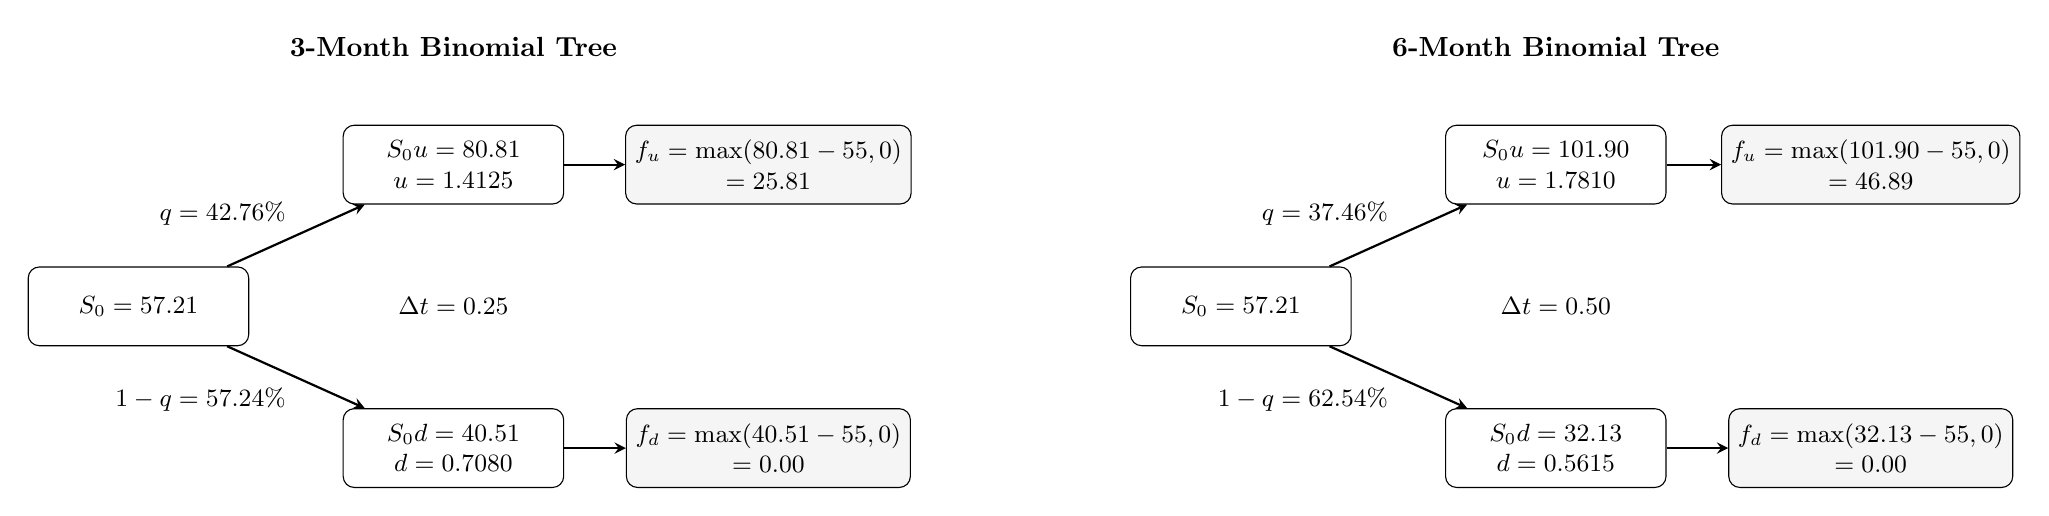
\begin{tikzpicture}[
    x=1cm,
    y=1cm,
    every node/.style={font=\small},
    state/.style={draw, rounded corners, align=center, minimum width=2.8cm, minimum height=1cm},
    payoff/.style={draw, rounded corners, align=center, minimum width=3.4cm, minimum height=1cm, fill=gray!8},
    title/.style={font=\bfseries},
    >=stealth
]
    \node[title] at (4,3.3) {3-Month Binomial Tree};
    \node[state] (s03) at (0,0) {$S_0=57.21$};
    \node[state] (su3) at (4,1.8) {$S_0u=80.81$\\$u=1.4125$};
    \node[state] (sd3) at (4,-1.8) {$S_0d=40.51$\\$d=0.7080$};
    \node[payoff] (fu3) at (8,1.8) {$f_u=\max(80.81-55,0)$\\$=25.81$};
    \node[payoff] (fd3) at (8,-1.8) {$f_d=\max(40.51-55,0)$\\$=0.00$};

    \draw[->, thick] (s03) -- node[above left] {$q=42.76\%$} (su3);
    \draw[->, thick] (s03) -- node[below left] {$1-q=57.24\%$} (sd3);
    \draw[->, thick] (su3) -- (fu3);
    \draw[->, thick] (sd3) -- (fd3);
    \node[align=center] at (4,0) {$\Delta t=0.25$};

    \node[title] at (18,3.3) {6-Month Binomial Tree};
    \node[state] (s06) at (14,0) {$S_0=57.21$};
    \node[state] (su6) at (18,1.8) {$S_0u=101.90$\\$u=1.7810$};
    \node[state] (sd6) at (18,-1.8) {$S_0d=32.13$\\$d=0.5615$};
    \node[payoff] (fu6) at (22,1.8) {$f_u=\max(101.90-55,0)$\\$=46.89$};
    \node[payoff] (fd6) at (22,-1.8) {$f_d=\max(32.13-55,0)$\\$=0.00$};

    \draw[->, thick] (s06) -- node[above left] {$q=37.46\%$} (su6);
    \draw[->, thick] (s06) -- node[below left] {$1-q=62.54\%$} (sd6);
    \draw[->, thick] (su6) -- (fu6);
    \draw[->, thick] (sd6) -- (fd6);
    \node[align=center] at (18,0) {$\Delta t=0.50$};
\end{tikzpicture}
}
\caption{Personalized one-step binomial trees for the 3-month and 6-month MP Materials Call valuation in Excel.}
\label{fig:tree}
\end{figure}

\section{Results Table \& Critical Conclusions}

\begin{table}[h]
\centering
\begin{tabular}{lcc}
\toprule
\textbf{Parameter} & \textbf{3-Month Analysis} & \textbf{6-Month Analysis} \\
\midrule
\textbf{Underlying \& Market Data} & & \\
Spot Price ($S_0$) & \$57.21 & \$57.21 \\
Strike Price ($K$) & \$55.00 & \$55.00 \\
Market Bid / Ask & \$9.45 / \$9.60 & \$12.25 / \$13.25 \\
\textbf{Market Mid-Price} & \textbf{\$9.53} & \textbf{\$12.75} \\
\midrule
\textbf{Model Inputs} & & \\
Annualized Volatility ($\sigma_Y$) & 69.07\% & 81.63\% \\
Risk-Free Rate (SOFR) & 3.68\% & 3.66\% \\
Capitalisation Factor & 1.0092 & 1.0183 \\
Discount Factor & 0.9909 & 0.9820 \\
\midrule
\textbf{Binomial Dynamics} & & \\
Up Factor ($u$) / Down Factor ($d$) & 1.4125 / 0.7080 & 1.7810 / 0.5615 \\
Risk-Neutral Prob. ($q$ / $1-q$) & 42.76\% / 57.24\% & 37.46\% / 62.54\% \\
Payoff Up ($f_u$) / Payoff Down ($f_d$) & \$25.81 / \$0.00 & \$46.89 / \$0.00 \\
\midrule
\textbf{Valuation \& Spread} & & \\
\textbf{Theoretical Price ($P_0$)} & \textbf{\$10.93} & \textbf{\$17.25} \\
Pricing Gap (Model Spread \$) & +\$1.41 & +\$4.50 \\
\textbf{Pricing Gap (Model Spread \%)} & \textbf{+14.79\%} & \textbf{+35.30\%} \\
\bottomrule
\end{tabular}
\caption{Consolidated Output: One-Step Binomial Model vs. Market Pricing.}
\label{tab:results}
\end{table}

The comparative analysis provides powerful insights into the mechanics of option pricing and the structural limitations of the One-Step Binomial Model when applied to high-volatility equities like MP Materials.

\subsection{Confirmation of the Time Value Principle}
The empirical results clearly demonstrate the fundamental principle of \textit{Time Value}. By extending the option's maturity from 3 to 6 months, the theoretical premium ($P_0$) increases significantly from \$10.93 to \$17.25. A longer time horizon grants the underlying asset more time to experience favorable volatility, which is geometrically reflected in the massive increase of the Up-Node payoff ($f_u$), soaring from \$25.81 (3-month) to \$46.89 (6-month).

\subsection{Divergence: Historical vs. Implied Volatility}
The most critical finding of this report is the systematic overvaluation of the options by the theoretical model, characterized by a positive pricing gap of +14.79\% for the 3-month contract and a substantial +35.30\% for the 6-month contract. 

This discrepancy highlights the fundamental difference between backward-looking and forward-looking risk metrics. The model was calibrated using \textbf{Historical Volatility} ($\sigma_Y$ of 69.07\% and 81.63\%), capturing a period of extreme market turbulence for MP Materials (evident from its wide 52-week range). However, the real market Mid-Prices (\$9.53 and \$12.75) are driven by \textbf{Implied Volatility}. The lower market premiums indicate that institutional investors and market makers expect the future price action of MP Materials to stabilize, thereby pricing in a lower volatility regime than what was observed in the past.

\subsection{Structural Limitations of the One-Step Framework}
Finally, the widening of the error margin in the 6-month analysis (+35.30\%) exposes the inherent limitations of a single-period binomial tree. Oversimplifying 6 months of continuous trading into a single discrete jump creates extreme, unrealistic terminal states. Specifically, the model assumes the stock will either surge by 78.1\% ($u=1.7810$) or crash by 43.8\% ($d=0.5615$) in exactly one step. In reality, option pricing over longer horizons requires multi-step lattices (e.g., 50 or 100 steps) or continuous-time models (Black-Scholes) to properly smooth the distribution of terminal prices and align theoretical values closer to market realities.

\end{document}